%!TEX root=/Users/rohitdholakia/Work/Thesis-Work/Thesis/thes-full.tex
%%%%%%%%%%%%%%%%%%%%%%%%%%%%%%%%%%%%%%%%%%%%%%%%%%%%
%
%     Chapter 3   
%
%%%%%%%%%%%%%%%%%%%%%%%%%%%%%%%%%%%%%%%%%%%%%%%%%

\chapter{Baselines}
\label{chap:baselines}

\section{Haitian-Creole}

\subsection{What is Haitian-Creole?}
	
	Creoles are languages that are a mixture of two or more languages. In general, there is a dominant language, which is the \emph{superstratum} and the other language is \emph{substratum}. Haitian-Creole is a French-based Creole, making French the superstratum language, and Fongbe, a West African language, is the substratum language. Superstratum is a language that is spoken by a small but powerful community ( like French in case of Haitian-Creole) and substratum is what is spoken by majority but common population. A creole comes about when the majority need to speak with the minority. So you get influences from both the classes~\cite{Claire:98}. Typically, the superstratum influences the grammar while the vocabulary has large influences from the substratum. This is observed in Haitian-Creole which has the same subject-verb-object behaviour as French, but the words in Haitian-Creole are different from French. Part of the reason behind the different vocabularies is that the French part of Haitian-Creole is not the Parisian French spoken and written today. Haitian-Creole has influences from 18th Century French, thus having words that might mean the same thing albeit spelt differently. There are several other instances of Creole in existence today, e.g, a form of French Creole is spoken in Quebec, Mauritian Creole is also a French-based Creole. Haitian-Creole has been in existence since quite sometime but became an official language of the Republic of Haiti only in 1961, alongwith French. \alert{Should we talk more about Haitian-Creole and some peculiar properties ? }


\subsection{Workshop on Haitian-Creole, 2011}
\label{sec:earthquake}

In January, 2010, a massive earthquake hit the country of Haiti. To provide relief and help to the masses, Mission 4636 set up a phone number ``4636'', where affected people could send messages about their location and ask for help. These were in Haitian Creole and were manually translated by volunteers who could speak the language. Each message had several tags, and depending on whether it was ``actionable'' or not, the help was provided.  After a week, Microsoft and Google released the first machine translation systems for Haitian-Creole. The effort of the volunteers, the initial MT systems by Microsoft and Google, with the data released by CMU, begged the question, \emph{``Can we use MT systems during Crisis ?''}. 

\subsection{Data}
\label{sec:baseline_data}



\subsection{OOD, Wiki and SMS}
	The training data available to us can be broadly divided into 3 categories, namely, out-of-domain(OOD), Wikipedia and SMS. OOD data comprises dictionaries and glossaries. Wikipedia data has parallel sentences and named entities from Wikipedia. And SMS data comprises raw short messages sent by people after the earthquake. The in-domain SMS data forms only 15\% of the training corpus. 

	The development, heldout and test sets comprise only short messages. Each have two versions, \emph{raw} and \emph{clean}. The \emph{raw} versions have the short message as-is while the clean versions have the same short messages, but manually cleaned up to remove spelling mistakes and punctuation symbols in the wrong places. \alert{Give an example}. 

	For instance, a short message sent might look like the one below : 

	\begin{verbatim}
		mwen BESWEN imfomasyon tou suit sou tan an.
	\end{verbatim}

	This is in the raw development file. The same message will look like the following post cleaning:

	\begin{verbatim}
		Mwen bezwen enfòmasyon touswit sou lameteyo.
	\end{verbatim}

	In the clean version, the words have the right case and the misspelt Haitian-Creole word imfomasyon is correctly spelt as enf\`{o}masyon. The same scenario is true for the heldout and test sets. In all our experiments, we will learn weights for our various translation model features using the clean version of the development set, but our aim is to improve the accuracy on the \emph{raw}, \emph{noisy} heldout and test sets. 

	Moreover, having development, heldout and test sets, all from the same niche domain, introduces more challenges. There is limited training data available between Haitian-Creole and any other language, including English, and the task is to improve the translations for a completely different domain in the form of Short Messages. Hence, on top of the low-resource challenge, we have a canonical Domain Adaptation problem. 


	\begin{figure}[ht]
		\small
		\centering
		\label{fig:haiti_data_settings}
		



\begin{tabular}{  lr  } \toprule

Data & \#lines  \\ 
\toprule
\emph{Test} \\
\cmidrule(r){1-2} 


dev & 900 \\
devtest & 900 \\
test & 1274 \\
\toprule
%\begin{comment}
\emph{Training} \\
\cmidrule(r){1-2} 
%Data & \#lines \\

SMS & 16000 \\
OOD & 87000 \\
Wiki & 11000 \\ 

%\begin{comment}


\bottomrule
\small
\label{table:datasets}
\end{tabular}


		\caption{Data Settings - Haitian-Creole}
	\end{figure}

To enable more research in low-resource languages like Haitian Creole, the messages sent to ``4636'' were released as part of the Sixth Workshop in Statistical Machine Translation in 2011. The task was to improve the translations on a test set comprising only Short Messages, both clean and raw. Clean test sets were manually cleaned by correcting misspelt and incomplete words. The training data comprises 15\% SMS with Wikipedia and other data sources forming the out-of-domain training corpus. Nine systems participated in the task. Various approaches were tried to deal with the low-resource scenario and some systems also tried to use French to handle the noise. 

\subsection{Workshop related work}
\alert{It was confusing to explain the data in related work. hence data came first}

 ~\cite{Sanjika:11} used spelling normalization to reduce the words with special characters to their nearest correct spelling, using a noisy-channel based spelling normalizer. Spelling of Haitian Creole words were corrected by using edit distance with French words as Haitian Creole is derived from 18th century French. For the edit distance, they generated a clean dictionary using the cleaner versions of the development and heldout  parts and if a word from the noisy side is not present in the cleaner corpus, then, the edit distance with the French words was used. Following the spelling normalization, Semantic role labeling was used to expand the corpus. They used a maximum-entropy classifier to extract parallel sentences from comparable corpora and then used a normalizer to get their best performing system from Haitian Creole - English. Note that the best system turns out to be their baseline system. Denoising by spell correction, using corpus expansion and automatic generation of parallel data reduces their BLEU score. 


 ~\cite{Vladimir:11} use a Hierarchical Phrase-based translation system. They observe that annotating beginning and end of sentence markers as part of the translation process significantly improves performance. Duplicating of data resources when you have limited parallel resources to start with helped. But, not all the OOD resources provided carry the same weightage. Some dictionaries, for instance, carry more weightage than parallel sentences from Wikipedia. Weighting of different parts of the corpora and duplicating some parts results in some BLEU score appreciation. They also explore the approach of using a finite-state automata to translate ``raw'' SMS to ``'clean'' SMS followed by the  translation pipeline but this does not help. Grammar filtering leads to the best performing system. 


 ~\cite{Hardmeier:11} only translate the clean versions of the heldout and test set. By generating word alignments using GIZA++ and transduction grammars allows the phrase table to pick the best out of the two, and they mainly concentrate \alert{bad word ?} on improving word alignments for phrase-based systems and determining if dependency parsing can be integrated into a syntax-based approach. They use two language models, a domain-specific language model generated using the English side of the Haitian-Creole to English corpus and a much larger Gigaword corpus. 



 ~\cite{Sara:11} reports the efficacy of various spell-correction techniques when used on the noisy side of the training corpus. The training corpus consists of raw Short Messages. One of the major challenges in the task was handling the noise present in the in-domain training data. Words like cafe were spelt as \textbf{caf*} sometimes as the messages were sent on  primitive typing pads. While some systems tried to use monolingual French corpora to reduce the misspelt words to their nearest forms,~\cite{Sara:11} used various spell correction techniques based on edit distances to achieve the same objective. 


 ~\cite{Banchs:11} propose to use the same SMT system for both raw and clean data.  They also stood first in the human evaluations conducted for the 9 participants.They make a SMT system to translate the raw,noisy SMS to clean SMS . They used the dev and test datasets to generate this,which have 900 sentences each. Note that they train a SMT system to translate noisy training SMS to a cleaner version by using the development, heldout and test sets as training. 







\section{Malagasy}
	Malagasy belongs to the Austronesian family and is the national language of Madagascar. It has a Latin script, is spoken by about 18 million people in the world. To our best knowledge, no previous work has addressed the challenges involved in having a SMT system for Malagasy. \alert{anything more about Malagasy ?maybe an example }
\subsection{Data}
	The data used is part of the global voices project\footnote[1]{http://www.ark.cs.cmu.edu/global-voices/}. Every month, new documents are released which have been translated by volunteers. 

	\begin{figure}[ht]
		\small
		\centering
		\begin{tabular}{l|r} 
			training & 88000 \\
			dev & 1133 \\
			heldout & 500 \\
			test & 633 \\
		\end{tabular}
		\caption{Data settings for Malagasy}
	\end{figure}

\subsection{Uniqueness}

\begin{verbatim}
haiti : rescuing survivors , searching for the missing
haiti : manavotra ny velona , mitady ny tsy hita 
\end{verbatim}
\section{BLEU(s)}
\label{sec:baseline_results}

\begin{figure}[h]
	\small
	\centering
	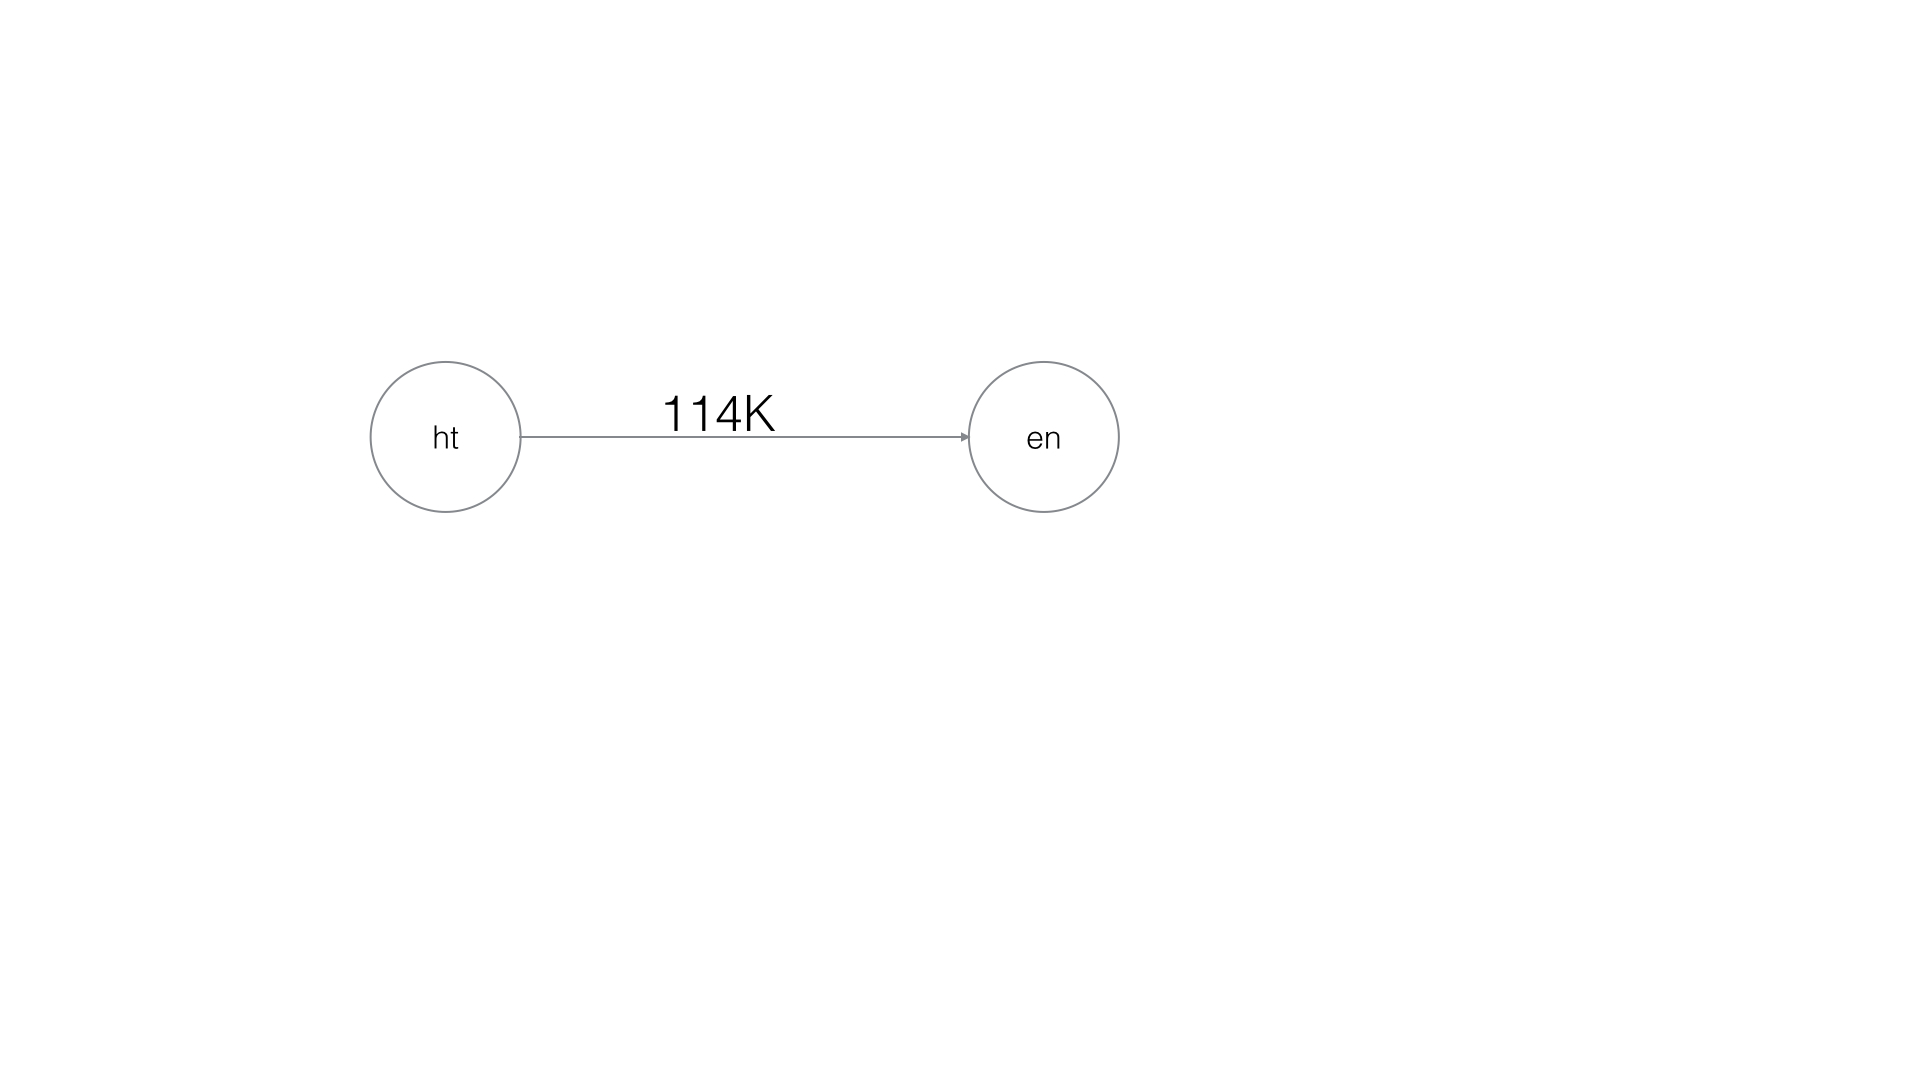
\includegraphics[trim=4cm 4cm 4cm 4cm, clip=true, totalheight=0.5\textheight]{files/Figures/baseline.jpg}
	\caption{Haitian Creole - English baseline}
	\label{fig:training}
\end{figure}

To better understand the effect of the in-domain part of the training data, we report baseline results using various parts of the data, alone and together. A direct Haitian-Creole to English system using just the 15\% of the in-domain training data comfortably beats direct systems trained on a lot more data, in terms of the number of lines, but out-of-domain data. Using all the parallel corpora available to us gives us the best BLEU of all. We also report our baseline using a much larger language model, called \emph{bigLM}. This language model is an interpolation of the English side of the WMT corpus with the english side of Europarl. In all the future experiments, we will use the full-bigLM as our baseline for comparison. 

\begin{figure}[ht]
	\small
	\centering
	\begin{tabular}{lllll} \toprule
System & d(cl) & d(r) & t(cl) & t(r) \\
\toprule
just-ood & 27.56 & 20.77 & 26.72 & 20.14 \\
just-sms & 32.85 & 29.15 & 32.09 & 27.56 \\
full & 33.52 & 29.76 & \emph{33.1} & 28.19 \\
full-bigLM & 33.6 & 29.83 & 33.07 & 28.91 \\ 
\bottomrule
\small
\centering
\label{table:baselines}
\end{tabular}

	\label{fig:haiti_baselines}
	\caption{Baselines - Haitian-Creole to English}
\end{figure}

\section{Mawukakan}
	Mawukakan is one of the four Mandekan languages, the other three being Bambara, Maninkakan and Wojenekakan. Mandekan languages are the Eastern Manding languages of the Mande group of the Niger-Congo family of languages and are small languages, spoken by only half a million people around the world. The Mandekan languages lack a written tradition and hence, have very little representation on the Internet. In this dissertation, we report our results on Maninkakan and Mawukakan to English systems, and the improvements observed when using French as a pivot language. 
	\begin{figure}[ht]
		\small
		\centering
		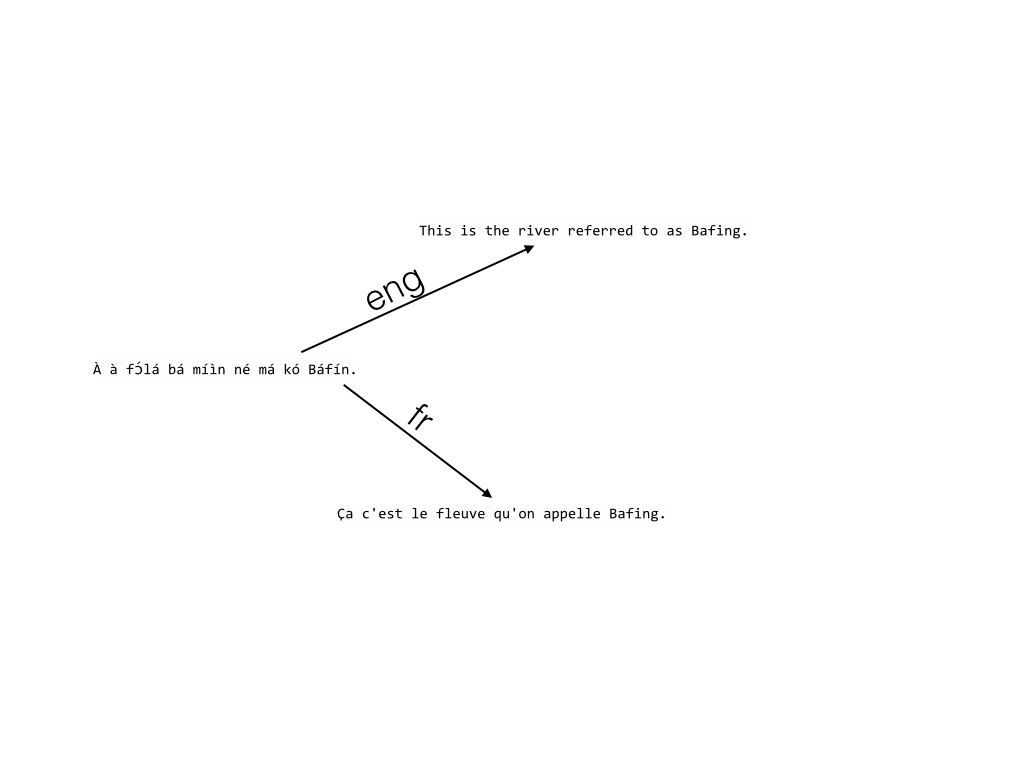
\includegraphics[trim=4cm 1cm 2cm 3cm, clip=true, height=0.6\textheight]{files/Figures/mawu.jpg}
		\caption{Example Mawu - English - French translation}
		\label{fig:mawu_example}
	\end{figure}
	
	\begin{figure}[ht]
		\small
		\centering
		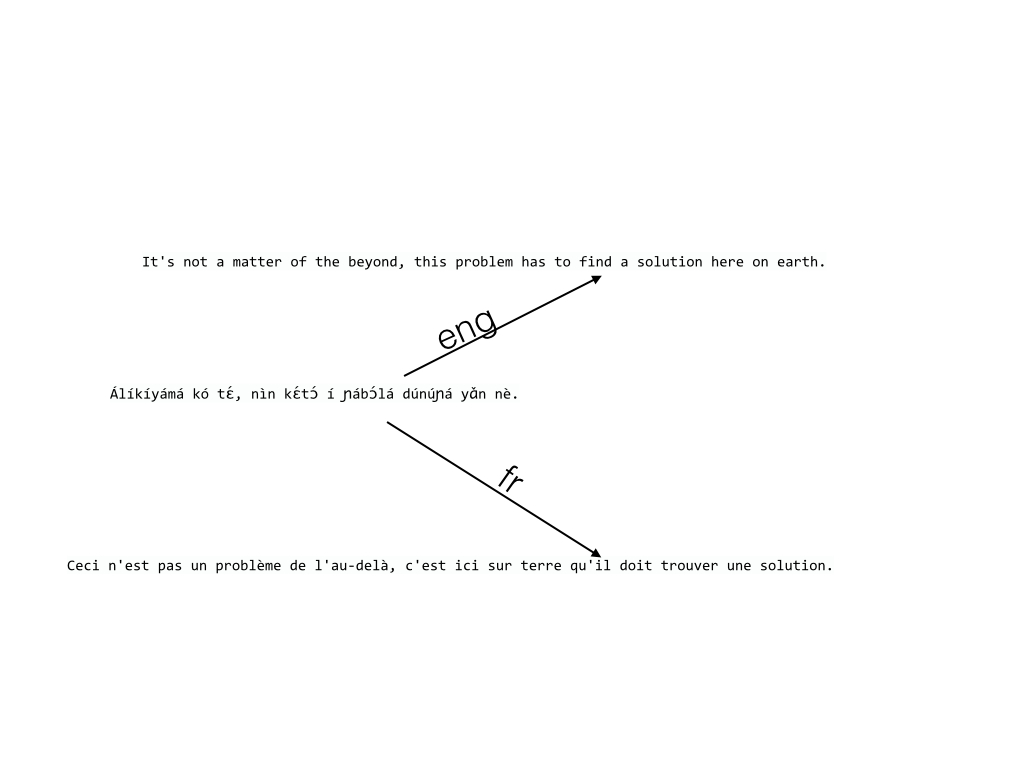
\includegraphics[trim=4cm 2cm 2cm 3cm, clip=true, height=0.6\textheight]{files/Figures/manin.jpg}
		\caption{Example Maninkakan - English - French translation}
		\label{fig:manin_example}
	\end{figure}
	



\section{Remarks}
\label{sec:baseline_remarks}



